\chapter{Название лабораторной работы}

\section{Цель работы}
Здесь приводится формулировка цели лабораторной работы. Формулировки цели для каждой лабораторной работы приведены в методических указаниях. 
В~курсе <<Языки и методы программирования>> используются методические указания \cite{gutgut:1, gutgut:2}.

Цель данного шаблона "--- максимально упростить подготовку отчётов по лабораторным работам в системе \href{https://ru.wikipedia.org/wiki/LaTeX}{\LaTeXe}. 
Модифицируя данный шаблон, студенты смогут без труда подготовить <<стильный>> и качественный (с точки зрения оформления и набора) отчёт по лабораторным работам, а также познакомиться с основными возможностями \LaTeXe, которые безусловно пригодятся при подготовке курсовых и дипломных проектов, оформлении научных статей, магистерских и даже кандидатских диссертаций. 
Для уверенного и <<продвинутого>> владения этой системой настоятельно рекомендуется ознакомиться хотя бы с~одной из этих книг \cite{latex:b1,latex:b2,latex:b3}, которые можно найти в электронном виде в сети Internet или спросить у преподавателя. 
Также можно пользоваться любыми материалами, найденными в сети.

\section{Задание}
Здесь приводится описание задания в соответствии с~рекомендациями методического пособия и~выданным вариантом~\cite{gutgut:1, gutgut:2}.

Студентам предлагается работать с издательской системой \LaTeXe, установленной не на настольном компьютере, а~в~облачном сервисе \href{http://www.overleaf.com}{Overleaf}. 
Это связано с~тем, что пользователю незнакомому с~\LaTeX\ порой весьма трудно самостоятельно установить, настроить и начать работать с этой системой.
Сервис \href{http://www.overleaf.com}{Overleaf} имеет удобный и понятный интерфейс, в нём всё работает <<из коробки>>.

Для начала работы с сервисом \href{http://www.overleaf.com}{Overleaf}  необходимо зарегистрироваться одним из следующих способов: 
\begin{itemize}
\item с помощью аккаунта \href{https://www.overleaf.com/users/auth/google_oauth2?intent=sign_up?ref=21785d9c7b53}{Google};
\item с помощью аккаунта \href{https://www.overleaf.com/users/auth/twitter?intent=sign_up?ref=21785d9c7b53}{Twitter}
\item или с помощью регистрации через  \href{https://www.overleaf.com/signup?ref=21785d9c7b53}{электронную почту}.
\end{itemize}

После регистрации можно открыть этот шаблон по ссылке \url{https://www.overleaf.com/read/sqvxbnhgxxdm} и начать оформлять отчёт по лабораторным работам.
Язык проверки орфографии "--- единственное, что следует изменить в~настройках этого сервиса: \href{https://www.overleaf.com/users/edit#!accountsettings}{Default Spell Check Language (for new projects)}.

На рис.~\ref{fig:overleaf} представлен  экран с тулбаром сервиса Overleaf.
Блок \colorbox{ForestGreen}{\color{white}\verb"PROJECT"}, предназначен для управления файлами проекта, в частности можно добавить и изменить файлы 
\fcolorbox{black}{lightgray}{\color{ForestGreen}Add files...}.
При работе с сервисом рекомендуется использовать режим \colorbox{ForestGreen}{\color{white}\texttt{Source}}, а не
\texttt{Rich Text}.

\begin{figure}[h!]
\centering
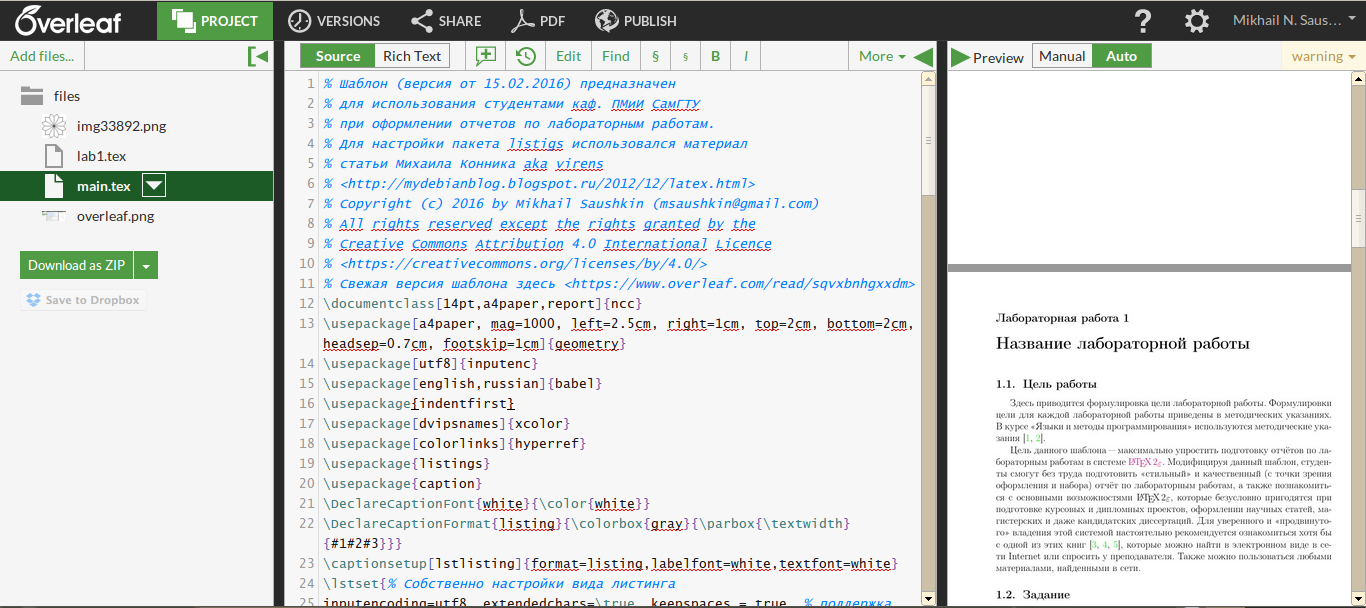
\includegraphics[width=.98\textwidth]{overleaf}

\caption{Экран с тулбаром сервиса Overleaf}
\label{fig:overleaf}
\end{figure}

\section{Основная часть}

\subsection{Теоретическая часть}

Здесь приводятся теоретические сведения, необходимые для выполнения соответствующей лабораторной работы: описываются методы решения поставленной задачи, используемые подходы, алгоритмы.

Преимущество \LaTeX{а} перед другими системами в том, что Вы можете набирать свой текст не задумываясь об оформлении. 
Система \LaTeXе\ всё сделает сама в~лучшем виде согласно настройкам, заданным в преамбуле документа, ведь создатель \TeX{а}  не кто иной, как \href{https://ru.wikipedia.org/wiki/%D0%9A%D0%BD%D1%83%D1%82,_%D0%94%D0%BE%D0%BD%D0%B0%D0%BB%D1%8C%D0%B4_%D0%AD%D1%80%D0%B2%D0%B8%D0%BD}{Дональд Кнут}, 
а макропакет \LaTeX\ разработал \href{https://ru.wikipedia.org/wiki/%D0%9B%D1%8D%D0%BC%D0%BF%D0%BE%D1%80%D1%82,_%D0%9B%D0%B5%D1%81%D0%BB%D0%B8}{Лесли Лэмпорт}.

Набор текста, формул и таблиц как правило не вызывает проблем, но в~первое время рекомендуется просматривать уже указанные книги~\cite{latex:b1,latex:b2,latex:b3}, написанные настоящими \href{https://ru.wikipedia.org/wiki/%D0%93%D1%83%D1%80%D1%83_(%D0%B7%D0%BD%D0%B0%D1%87%D0%B5%D0%BD%D0%B8%D1%8F)}{гуру} \LaTeX{а}.

\subsection{Листинг программы}

Листинг программы оформляется с помощью пакета \verb"listings". 
Документация по этому пакету очень обширная, её можно найти по ссылке \url{http://mirrors.ctan.org/macros/latex/contrib/listings/listings.pdf}.
Рекомендуется использовать настройки пакета уже прописанные в данном шаблоне в~преамбуле документа. 
Ниже представлен листинг программы~\ref{listing1} для чтения типизированного файла, взятый из методического пособия~\cite{gutgut:1}, оформленный в~соответствии с прописанными настройками.

\begin{lstlisting}[label=listing1, caption=Программа чтения типизированного файла]
const
	Nmax = 10;
type
	TCircle = record
		x, y, R : integer;
		color : string[20];
	end;
var
	W : array[1..Nmax] of TCircle;
	i, N, min, max : integer;
	f : file of TCircle;
begin
	// открываем файл для чтения
	Assign(f, '0.dbf'); Reset(f);
	N := FileSize(f);;
	for i:=1 to N do begin
		Read(f,W[i]);
	end;
	Close(f);
	max := -MaxInt;
	min := MaxInt;
	for i:=1 to N do begin
		if (W[i].color='зелёный') and (W[i].R>max) then max := W[i].R;
		if (W[i].color='красный') and (W[i].R<min) then min := W[i].R;
  	end;
  	if max = -MaxInt then Writeln('Зелёных кругов нет')
  		else Writeln('Радиус самого большого зелёного круга = ', max);
	if min = MaxInt then Writeln('Красных кругов нет')
		else Writeln('Радиус самого маленького красного круга = ', min);
end.
\end{lstlisting}

В случае, если для выполнения поставленного задания необходимо написать две программ, то приводятся листинги обеих программ.

При необходимости даются комментарии к листингам. Например, в листинге~\ref{listing1} в разделе типов задаётся тип \verb"TCircle", который используется для хранения данных:
\begin{verbatim}
type
	TCircle = record
      x, y, R : integer;
      color : string[20];
    end;
\end{verbatim}

\subsection{Полученные результаты и их анализ}

Здесь кратко описываются итоги проделанной работы, приводится анализ полученных результатов.

Здесь могут содержаться листинги входных и выходных файлов, приводиться таблицы и рисунки, используемые при анализе.

Пример оформления таблицы представлен ниже (см. табл.~\ref{tabl:1}). Она взята из указанного уже методического пособия~\cite{gutgut:1}.

\begin{center}
\begin{table}[h!]
\centering
\caption{Исходные данные для рассматриваемой задачи}
\label{tabl:1}
\begin{tabular}{|c|c|c|c|c|}
\hline
Номер &~~~~$X$~~~~ &~~~~$Y$~~~~&~~~~$R$~~~~&~~~~Цвет~~~~\\
\hline
1 &	100  &	170 & 30 & \color{red} красный\\
2 &	100  &	90	& 60 & \color{yellow} жёлтый\\
3 &	230  &	250	& 50 & \color{blue} синий\\
4 &	130  &	240 & 60 & \color{green} зелёный\\
5 & 300  &	130 & 30 & \color{green} зелёный\\
6 &	200  &	150	& 90 & \color{red} красный\\
\hline
\end{tabular}
\end{table}
\end{center}

Как отмечалось выше, рисунки также могут быть вставлены в отчёт, если они необходимы. См., например, рис.~\ref{fig:1}.

\begin{figure}[h!]
\centering

\includegraphics[scale=1.0]{img33892}

\caption{Задание к одному из вариантов, взятое из методических указаний~\cite{gutgut:2}}
\label{fig:1}
\end{figure}

Подробную информацию о том, как вставлять рисунки и таблицы в документ, также можно найти в уже упоминавшейся литературе~\cite{latex:b1,latex:b2,latex:b3}. 

\section{Выводы}
Здесь кратко описываются итоги проделанной работы.

В настоящем шаблоне заложены основы продуктивной работы в системе \LaTeXe.  Конечно в столь кратком изложении не возможно показать всю мощь и красоту \LaTeX{а}. 
<<Нужно сказать, что \LaTeX\ является \href{https://ru.wikipedia.org/wiki/%D0%9F%D0%BE%D0%BB%D0%BD%D0%BE%D1%82%D0%B0_%D0%BF%D0%BE_%D0%A2%D1%8C%D1%8E%D1%80%D0%B8%D0%BD%D0%B3%D1%83}{Turing complete language}, то есть на нем можно писать любые программы. Например, можно написать \href{http://tug.org/TUGboat/tb11-3/tb29greene.pdf}{интерпретатор Бейсика}, \href{http://en.literateprograms.org/Turing_machine_simulator_%28LaTeX%29}{симулятор машины Тьюринга}, 
\href{http://www.thole.org/manfred/apfel/}{Mandelbrot with LaTeX} и \href{http://stackoverflow.com/questions/2968411/ive-heard-that-latex-is-turing-complete-are-there-any-programs-written-in-late}{другие программы}. То есть на латехе можно писать что угодно.>>\footnote{Фраза взята вот отсюда: \url{http://mydebianblog.blogspot.ru/2013/12/latex.html}.}

\vfill
\centerline{\Huge Happy \TeX{ing}!}
\vfill
